% =====================================================================
\section{Simulation Results}\label{sec:experiments}
% =====================================================================
This section evaluates the proposed tactical--planning--control hierarchy in
the semi-physical simulation environment used by the Abu Dhabi Autonomous
Racing League (A2RL).  The evaluation is organized as follows.  First, the
hardware-in-the-loop simulation environment and the communication interface
are described.  Second, all numerical parameters used by the vehicle model,
tactical layer, planner, learning module, and controller are consolidated in a
single table.  Two representative overtaking cases are then analyzed in
detail, followed by an aggregate 1000-lap validation.

\subsection{Semi-Physical A2RL Simulation Environment}
\label{subsec:hil_env}
The closed-loop experiments were carried out in the official simulator
developed by the A2RL race organizer.  The simulator provides the Yas Marina
track geometry, the Dallara EAV24 vehicle interface, the opponent vehicle, and
the race-control message stream.  The planner and controller were not coupled
to the simulator through direct function calls.  Instead, the software stack
communicated with the virtual vehicle platform through a virtual CAN channel,
using the same message abstraction as the race vehicle interface.  Sensor
states, opponent states, race-control flags, and vehicle feedback were received
from the simulator, while planned actuation commands were returned through the
same virtual CAN loop.

This configuration is a semi-physical simulation rather than a purely
algorithmic benchmark: the decision stack runs as an external real-time
process, all inter-layer and vehicle-interface timing must survive the message
transport layer, and the controller receives only the state variables exposed
by the platform interface.  Consequently, failures caused by delayed tactical
updates, infeasible planner outputs, or controller fallback logic appear in the
closed loop exactly as they would in the vehicle software stack.  The
experiments therefore test not only whether an overtake trajectory exists, but
whether the learned corridor, the SOCP planner, the speed profiler, and the
MPCC controller remain mutually executable under the simulator's virtual-CAN
timing and race-control constraints.

\subsection{Parameter Configuration}
\label{subsec:param_setup}
All numerical parameters used in the experiments are summarized in
Table~\ref{tab:setup_params}.  The table intentionally reports only symbols
and values so that the implementation settings can be inspected without
interrupting the method derivations in the preceding sections.

\begin{table}[!htbp]
\centering
\scriptsize
\setlength{\tabcolsep}{2.2pt}
\renewcommand{\arraystretch}{1.12}
\caption{Parameter setting summary.}
\label{tab:setup_params}
\resizebox{\linewidth}{!}{%
\begin{tabular}{@{}lc|lc|lc|lc|lc@{}}
\toprule
Sym. & Val. & Sym. & Val. & Sym. & Val. & Sym. & Val. & Sym. & Val. \\
\midrule
$m$ & $742\,\mathrm{kg}$ &
$l_f,l_r$ & $1.75,\,1.35\,\mathrm{m}$ &
$I_z$ & $1500\,\mathrm{kg\,m^2}$ &
$C_f,C_r$ & $2.30,\,2.40{\times}10^5\,\mathrm{N/rad}$ &
$\mu$ & $1.20$ \\
$\delta_{\max}$ & $0.342\,\mathrm{rad}$ &
$\dot\delta_{\max}$ & $0.5\,\mathrm{rad/s}$ &
$[\underline a,\overline a]$ & $[-5,8]\,\mathrm{m/s^2}$ &
$v_{x,\max}$ & $90\,\mathrm{m/s}$ &
$\varepsilon_v$ & $0.5\,\mathrm{m/s}$ \\
$c_{d,2}$ & $-1.04765\,\mathrm{N\,s^2/m^2}$ &
$c_{d,1}$ & $47.5\,\mathrm{N\,s/m}$ &
$c_{d,0}$ & $-1609.73\,\mathrm{N}$ &
$p$ & $0.75$ &
$T_s$ & $0.05\,\mathrm{s}$ \\
$V_{\rm char}$ & $80\,\mathrm{m/s}$ &
$n_{\rm char}$ & $8\,\mathrm{m}$ &
$a_{\rm char}$ & $20\,\mathrm{m/s^2}$ &
$\Delta s_{\rm char}$ & $50\,\mathrm{m}$ &
$\Delta V_{s,\rm char}$ & $30\,\mathrm{m/s}$ \\
$g_{\rm char}$ & $50\,\mathrm{m}$ &
$\tau_{\rm tc,\max}$ & $30\,\mathrm{s}$ &
$\varepsilon_\tau$ & $0.01\,\mathrm{m/s}$ &
$L_t^{\rm cap}$ & $[1.5,6.0]$ &
$R_t^{\rm cap}$ & $[1.5,6.0]$ \\
$d_{\rm safe}$ & $[0.2,0.8]$ &
$V_{\rm cap}$ & $[15,90]$ &
$g_{\rm chase}$ & $[18,24]$ &
$g_{\rm ot}$ & $[16,24]$ &
$g_{\rm abort}$ & $[28,45]$ \\
$b_{\rm lat}$ & $[-1.5,1.5]$ &
$w_{\rm safe}$ & $[1,5]$ &
$q_{\rm side}$ & $[-1,1]$ &
$g_{\rm def}^{\rm front}$ & $25\,\mathrm{m}$ &
$g_{\rm def}^{\rm rear}$ & $20\,\mathrm{m}$ \\
$\Delta n_{\rm safe}$ & $2.5\,\mathrm{m}$ &
$g_{\rm interlock}$ & $6\,\mathrm{m}$ &
$T_{\rm imm}$ & $30\,\mathrm{s}$ &
$\phi_{\rm ot}$ & $30$ &
$\phi_{\rm ovb}$ & $-20$ \\
$\phi_{\rm col}$ & $-100$ &
$\phi_{\rm lat}$ & $-2$ &
$\phi_{\rm crush}$ & $-5$ &
$\phi_{\rm app}$ & $3$ &
$\phi_{\rm sm}$ & $-0.1$ \\
$\phi_{\rm gs}$ & $-0.5$ &
$\phi_{\rm sbs}$ & $0.5$ &
$\phi_{\rm wide}$ & $0.25$ &
$\alpha_Q$ & $3{\times}10^{-4}$ &
$|\mathcal{D}|$ & $10^5$ \\
$B$ & $256$ &
$\gamma$ & $0.99$ &
$\tau$ & $5{\times}10^{-3}$ &
$f_{\rm feat}$ & $51{\to}256{\to}256$ &
$f_{\pi,Q}$ & $[256,256]$ \\
$N_q$ & $25$ &
$K$ & $20$ &
$d_p$ & $300\,\mathrm{m}$ &
$N_{\rm sta}$ & $150$ &
$\Delta s_{\rm sta}$ & $2\,\mathrm{m}$ \\
$p_{\rm fade}$ & $3$ &
$S_{\rm fade}$ & $50\,\mathrm{m}$ &
$W_{\rm fun}$ & $2.5\,\mathrm{m}$ &
$W_{\rm near}$ & $5\,\mathrm{m}$ &
$\lambda_{\rm side}$ & $0.6$ \\
$L_{\min}^{\rm corr}$ & $3\,\mathrm{m}$ &
$\beta$ & $0.2$ &
$k_{\rm blend}$ & $9$ &
$d_{\rm rmp}$ & $40\,\mathrm{m}$ &
$k_{\rm sr}$ & $15$ \\
$q_l$ & $50$ &
$q_\psi$ & $5$ &
$q_v$ & $1$ &
$R_a$ & $0.05$ &
$R_{\dot\delta}$ & $30$ \\
$q_{\rm prog}$ & $0.5$ &
$w_\zeta$ & $1000$ &
$N_c$ & $15$ &
$T_c$ & $0.05\,\mathrm{s}$ &
$T_cN_c$ & $0.75\,\mathrm{s}$ \\
\bottomrule
\end{tabular}%
}
\end{table}

\subsection{Scenario I: Short Fast-Closure Overtake}
\label{subsec:case2}
The first scenario is a short fast-closure pass.  The ego vehicle enters the
engagement with a large closing-speed advantage and must convert this
advantage into a feasible lateral corridor before reaching the opponent.  The
run completes the pass with $\min\Delta s=-0.48\,\mathrm{m}$,
$\Delta t_{\rm pass}=1.13\,\mathrm{s}$ after entering \textsc{Overtake},
$\max V=73.10\,\mathrm{m/s}$, $\mathrm{RMS}(e_l)=0.02\,\mathrm{m}$,
$\mathrm{RMS}(e_v)=0.26\,\mathrm{m/s}$, and tactical gain
$\Delta\Gamma=1.38$.

\begin{figure}[H]
\centering
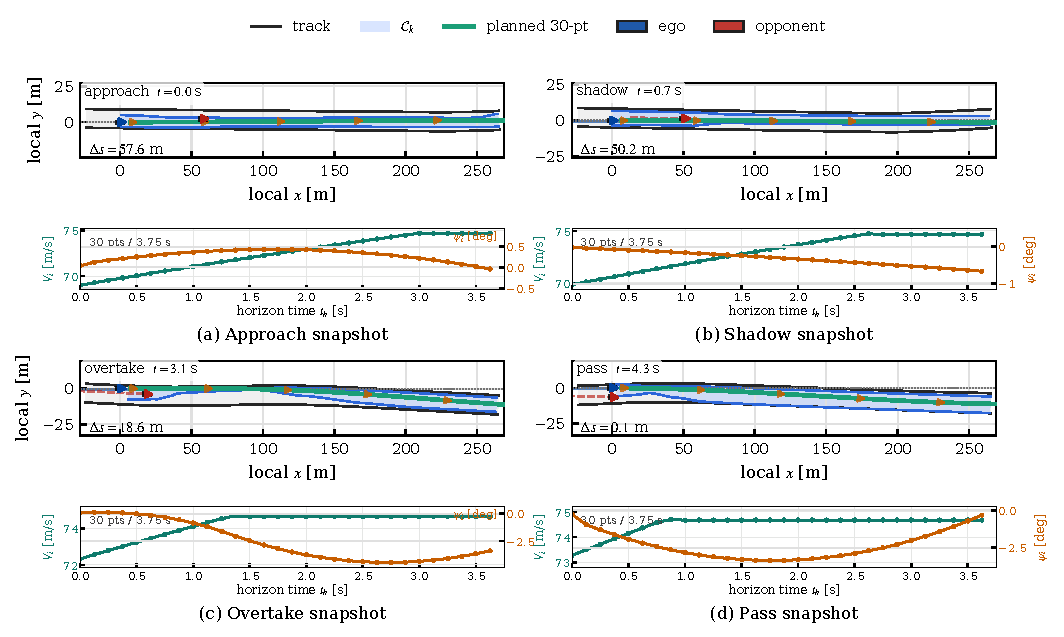
\includegraphics[width=\linewidth]{figures/case_02_engagement_snapshots.pdf}
\caption{Scenario~I engagement snapshots.  The four representative instants
show the planned tactical corridor and the local trajectory during approach,
shadowing, commitment, and pass completion.}
\label{fig:case02_engagement}
\end{figure}

Figure~\ref{fig:case02_engagement} shows that the tactical decision is made
before the vehicles become geometrically interlocked.  In the first snapshot,
the ego vehicle remains on a high-speed closure trajectory while the planner
keeps the corridor centered enough to preserve recoverability.  The second
snapshot corresponds to the shadowing phase: the feasible set begins to open
toward the selected pass side, but the corridor still contains a conservative
fallback around the raceline.  In the third snapshot, the FSM has committed to
\textsc{Overtake}; the corridor carver excludes the opponent footprint and
forces the SOCP path to occupy the free side of the track.  The final snapshot
shows the pass completion, where the planned path has cleared the opponent
without a discontinuous lateral jump.  This progression is important because
the learned component never commands steering or acceleration directly; it
only reshapes the feasible set that the deterministic planner and MPCC must
execute.

\begin{figure}[H]
\centering
\subfloat[Path and corridor.]{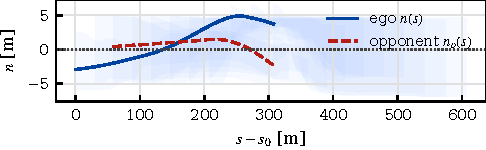
\includegraphics[width=0.48\linewidth]{figures/case_02_path_corridor.pdf}}
\hfill
\subfloat[Speed.]{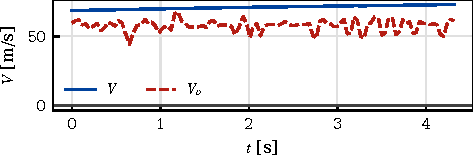
\includegraphics[width=0.48\linewidth]{figures/case_02_dynamics_speed.pdf}}\\[-1mm]
\subfloat[Acceleration.]{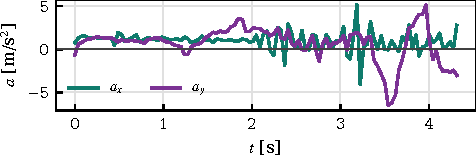
\includegraphics[width=0.48\linewidth]{figures/case_02_dynamics_accel.pdf}}
\hfill
\subfloat[Heading error.]{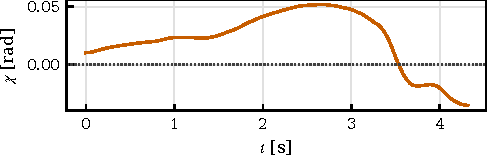
\includegraphics[width=0.48\linewidth]{figures/case_02_dynamics_heading.pdf}}
\caption{Scenario~I closed-loop execution states.}
\label{fig:case02_execution_grid}
\end{figure}

Figure~\ref{fig:case02_execution_grid} quantifies the dynamic execution of the
short pass.  The path plot confirms that the ego trajectory remains inside the
tactical corridor during the entire engagement, so the learned side decision
does not create a geometric constraint violation.  The speed trace reaches
$73.10\,\mathrm{m/s}$, indicating that the planner preserves the fast-closure
advantage rather than sacrificing it through excessive caution.  The
longitudinal and lateral acceleration histories remain smooth during the
transition into \textsc{Overtake}, which shows that the GG-constrained speed
profiler and MPCC friction slack prevent the maneuver from becoming a
bang--bang lateral escape.  The heading-error response stays bounded while
the lateral path changes side, demonstrating that the corridor transition is
converted into a controllable yaw demand rather than an abrupt heading
correction.

\begin{figure}[H]
\centering
\subfloat[Lateral tracking error.]{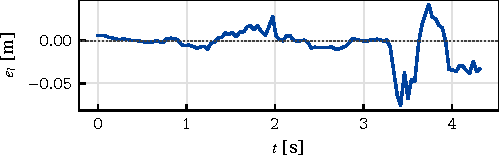
\includegraphics[width=0.48\linewidth]{figures/case_02_tracking_lateral.pdf}}
\hfill
\subfloat[Speed tracking error.]{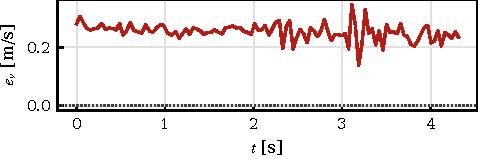
\includegraphics[width=0.48\linewidth]{figures/case_02_tracking_speed.pdf}}\\[-1mm]
\subfloat[FSM mode.]{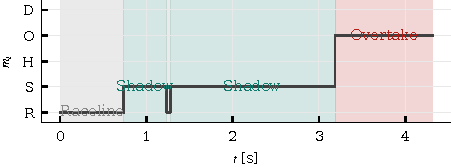
\includegraphics[width=0.48\linewidth]{figures/case_02_fsm_mode.pdf}}
\hfill
\subfloat[Corridor caps and side.]{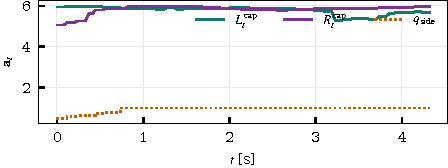
\includegraphics[width=0.48\linewidth]{figures/case_02_fsm_corridor.pdf}}
\caption{Scenario~I tracking and tactical-state responses.}
\label{fig:case02_tactical_grid}
\end{figure}

Figure~\ref{fig:case02_tactical_grid} shows that the controller tracks the
planner output with sub-decimeter accuracy despite the very short decision
window.  The lateral error has an RMS value of only $0.02\,\mathrm{m}$, so the
vehicle remains effectively on the planned path during the pass.  The speed
tracking error is also small, with $\mathrm{RMS}(e_v)=0.26\,\mathrm{m/s}$,
which confirms that the velocity cap and the GG sweep are consistent with the
MPCC's achievable acceleration envelope.  The FSM mode plot shows a clean
transition through \textsc{Shadow} and \textsc{Overtake}, while the corridor
plot shows that the committed side is held during the pass rather than
oscillating between alternatives.  This stable side commitment is the key
reason the planner can exploit the brief overtake opportunity without
inducing high-frequency replanning.

\subsection{Scenario II: Long Side-by-Side Overtake}
\label{subsec:case5}
The second scenario is a longer fast-closure pass in which the ego vehicle
must remain side-by-side with the opponent for a longer interval before
clearing it.  The run completes the pass with
$\min\Delta s=-0.84\,\mathrm{m}$, $\Delta t_{\rm pass}=8.63\,\mathrm{s}$,
$\max V=65.83\,\mathrm{m/s}$, $\mathrm{RMS}(e_l)=0.05\,\mathrm{m}$,
$\mathrm{RMS}(e_v)=1.82\,\mathrm{m/s}$, and tactical gain
$\Delta\Gamma=1.75$.

\begin{figure}[H]
\centering
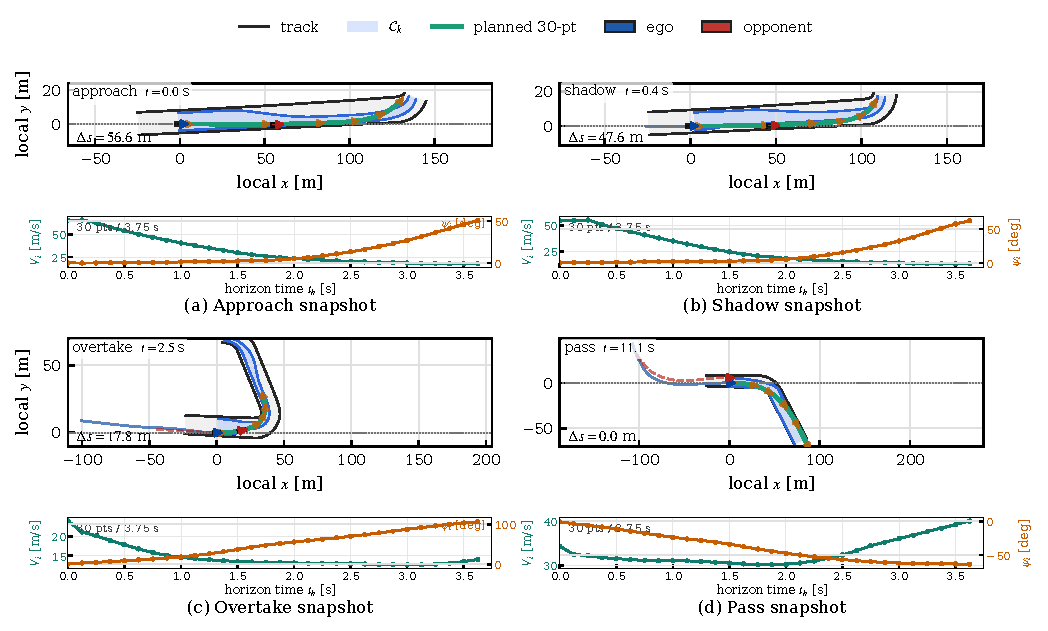
\includegraphics[width=\linewidth]{figures/case_05_engagement_snapshots.pdf}
\caption{Scenario~II engagement snapshots.  The four representative instants
show the planned tactical corridor and the local trajectory during the
extended side-by-side overtake.}
\label{fig:case05_engagement}
\end{figure}

Figure~\ref{fig:case05_engagement} illustrates a qualitatively different
engagement from Scenario~I.  The first instant shows the ego vehicle closing
from behind while the corridor remains broad enough to retain both tactical
options.  The second instant captures the onset of lateral displacement: the
planner starts to bias the path toward the selected side, but the speed
profile remains conservative enough to avoid forcing an infeasible overlap
with the opponent.  During the third instant, the vehicles are side-by-side;
the corridor excludes the opponent while preserving a continuous tube for the
SOCP path.  The fourth instant shows the ego vehicle ahead of the opponent,
with the tactical layer relaxing the corridor after the pass.  The sequence
demonstrates that the same hierarchy handles not only short impulse-like
passes, but also prolonged interactions where the corridor must remain stable
for several seconds.

\begin{figure}[H]
\centering
\subfloat[Path and corridor.]{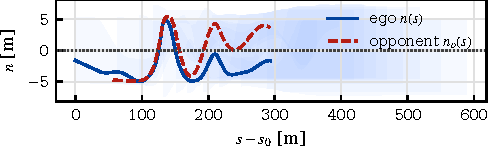
\includegraphics[width=0.48\linewidth]{figures/case_05_path_corridor.pdf}}
\hfill
\subfloat[Speed.]{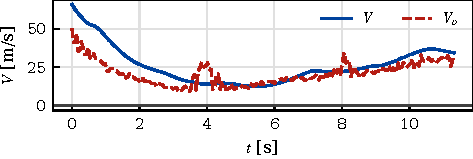
\includegraphics[width=0.48\linewidth]{figures/case_05_dynamics_speed.pdf}}\\[-1mm]
\subfloat[Acceleration.]{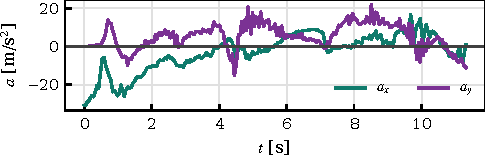
\includegraphics[width=0.48\linewidth]{figures/case_05_dynamics_accel.pdf}}
\hfill
\subfloat[Heading error.]{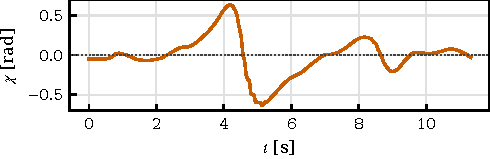
\includegraphics[width=0.48\linewidth]{figures/case_05_dynamics_heading.pdf}}
\caption{Scenario~II closed-loop execution states.}
\label{fig:case05_execution_grid}
\end{figure}

Figure~\ref{fig:case05_execution_grid} shows that the longer engagement is
executed with a lower peak speed of $65.83\,\mathrm{m/s}$, reflecting the
planner's need to remain in a viable side-by-side corridor rather than
complete an immediate speed-dominant pass.  The path remains inside the
carved corridor, which confirms that the tactical layer maintains a feasible
spatial tube even when the opponent occupies the critical region for a longer
time.  The acceleration plot shows larger dynamic transients than Scenario~I,
as expected for an extended interaction, but the response remains smooth
enough for the MPCC to track without friction-limit divergence.  The heading
response remains bounded during the side-by-side phase, indicating that the
SOCP path regularization prevents the lateral maneuver from degenerating into
a sharp steering correction.

\begin{figure}[H]
\centering
\subfloat[Lateral tracking error.]{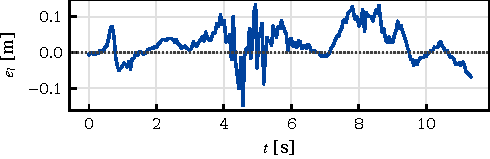
\includegraphics[width=0.48\linewidth]{figures/case_05_tracking_lateral.pdf}}
\hfill
\subfloat[Speed tracking error.]{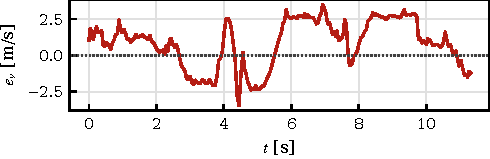
\includegraphics[width=0.48\linewidth]{figures/case_05_tracking_speed.pdf}}\\[-1mm]
\subfloat[FSM mode.]{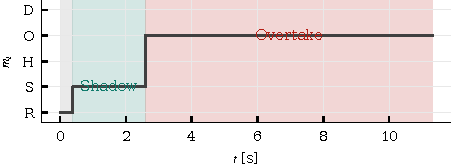
\includegraphics[width=0.48\linewidth]{figures/case_05_fsm_mode.pdf}}
\hfill
\subfloat[Corridor caps and side.]{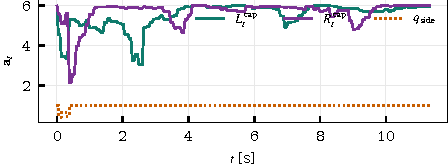
\includegraphics[width=0.48\linewidth]{figures/case_05_fsm_corridor.pdf}}
\caption{Scenario~II tracking and tactical-state responses.}
\label{fig:case05_tactical_grid}
\end{figure}

Figure~\ref{fig:case05_tactical_grid} confirms that the increased duration of
the duel does not destabilize the hierarchy.  The lateral RMS tracking error
is $0.05\,\mathrm{m}$, still well below the corridor width and therefore small
relative to the available passing margin.  The speed error increases to
$1.82\,\mathrm{m/s}$ because the controller must reconcile the speed profile
with a longer side-by-side geometry, but the error remains bounded and does
not prevent pass completion.  The FSM plot shows a persistent
\textsc{Overtake} tenure rather than rapid mode switching, and the corridor
plot shows a stable committed side throughout the decisive interval.  This is
the desired behavior for a learned tactical layer: once the policy selects a
pass side, the downstream solvers receive a consistent feasible set long
enough to execute the maneuver.

\subsection{Simulation Summary}
\label{subsec:sim_summary}
The two detailed scenarios expose complementary operating regimes.  Scenario~I
tests whether the hierarchy can exploit a short closing-speed opportunity,
whereas Scenario~II tests whether the same architecture can maintain a stable
side commitment during a longer side-by-side contest.  Table~\ref{tab:selected_overtake_metrics}
summarizes the closed-loop metrics of these two runs.

\begin{table}[!htbp]
\centering
\scriptsize
\setlength{\tabcolsep}{3.5pt}
\renewcommand{\arraystretch}{1.1}
\caption{Closed-loop metrics for the representative overtake scenarios.}
\label{tab:selected_overtake_metrics}
\begin{tabular}{@{}lccccc@{}}
\toprule
Case & $\Delta t_{\rm pass}$ & $\max V$ & RMS$(e_l)$ & RMS$(e_v)$ & $\Delta\Gamma$\\
 & [s] & [m/s] & [m] & [m/s] & [-]\\
\midrule
Scenario~I & 1.13 & 73.10 & 0.02 & 0.26 & 1.38 \\
Scenario~II & 8.63 & 65.83 & 0.05 & 1.82 & 1.75 \\
\bottomrule
\end{tabular}
\end{table}

Beyond the two representative cases, the same frozen tactical policy,
planner, and controller were evaluated over 1000 closed-loop laps in the
A2RL simulator.  No online learning, case-specific retuning, or controller
weight adjustment was used during this validation.  The aggregate results are
reported in Table~\ref{tab:aggregate_validation}.  The overtake success rate
of $94.7\%$ indicates that the learned tactical layer generalizes across a
large number of repeated race interactions while preserving compatibility with
the model-based planner and controller.  Equally important, the validation was
performed through the virtual-CAN semi-physical interface, so successful laps
reflect end-to-end timing consistency rather than offline trajectory
feasibility alone.

\begin{table}[!htbp]
\centering
\scriptsize
\setlength{\tabcolsep}{4pt}
\renewcommand{\arraystretch}{1.1}
\caption{Aggregate semi-physical validation results.}
\label{tab:aggregate_validation}
\begin{tabular}{@{}lc@{}}
\toprule
Metric & Value \\
\midrule
Closed-loop laps & $1000$ \\
Successful overtake laps & $947$ \\
Non-successful terminations & $53$ \\
Overtake success rate & $94.7\%$ \\
Online learning during validation & No \\
Case-specific controller retuning & No \\
\bottomrule
\end{tabular}
\end{table}

Overall, the experiments support the central design principle of the paper:
learning is most effective when it determines the tactical feasible set, while
the planner and controller enforce geometric consistency, handling-limit speed
selection, and closed-loop vehicle execution.  The short-pass and long-pass
cases show that the architecture is not tuned to a single overtaking geometry,
and the 1000-lap validation demonstrates that this separation remains robust
under repeated semi-physical simulation.
